\documentclass{cornouaille}
\dscornouaille

\begin{document}

\cornouaille{TS}{Devoir Surveillé 5}{Lundi 30 janvier 2019}

\Bareme


\encadre{
Le sujet est composé d'un certain nombre d'exercices indépendants.Vous devez traiter tous les exercices.\\
Pour chaque exercice, vous pouvez admettre un résultat précédemment donné dans le texte pour aborder les questions suivantes, à condition de l'indiquer clairement sur la copie.\\
Vous êtes invités à faire figurer sur votre copie toute trace de recherche, même incomplète ou non fructueuse, que vous aurez développée.\\
Il est rappelé que la qualité de la rédaction, la clarté et la précision des raisonnements seront prises en compte dans l'appréciation des copies.\\
}



:::exercice Exercice:

[Les complexes sont nos amis][5.5]
Le plan est muni d'un repère orthonormé $\left(\text{O};~\overrightarrow{u},~\overrightarrow{v}\right)$.

\smallskip

Les points A, B et C ont pour affixes respectives $a = - 4,\: b = 2$ et $c = 4$.

\medskip


\begin{enumerate}
\item On considère les trois points A$'$, B$'$ et C$'$ d'affixes respectives $a'= \text{j}a$, $b'= \text{j}b$ et $c'= \text{j}c$ où j est le nombre complexe:

$$
j=-\dfrac{1}{2} + \text{i}\dfrac{\sqrt{3}}{2}
$$


\begin{enumerate}
\item Donner la forme trigonométrique et la forme exponentielle de j.

\setbar{1.5}

:::startsolution

$\text{j}=-\dfrac{1}{2} + \text{i}\dfrac{\sqrt{3}}{2}=\cos\left(\dfrac{2\pi}{3}\right) + \text{i}\sin\left(\dfrac{2\pi}{3}\right)=e^{\frac{2\text{i}\pi}{3}}$

$a'=a\text{j}=-4\text{j}=2-2\text{i}\sqrt{3}=4\left( -e^{\frac{2\text{i}\pi}{3}}\right)=4\left( e^{\text{i}\pi}{\frac{2\text{i}\pi}{3}}\right)=4e^{\text{i}\left( \pi+\frac{2\pi}{3}\right)  }=4e^{\frac{5\text{i}\pi}{3}}=4e^{-\frac{\text{i}\pi}{3}}$

$b'= b\text{j}=2\text{j}=-1+\text{i}\sqrt{3}=2e^{\frac{2\text{i}\pi}{3}}$

$c'= c\text{j}=4\text{j}=-2+2\text{i}\sqrt{3}=4e^{\frac{2\text{i}\pi}{3}}$


:::endsolution

En déduire les formes algébriques et exponentielles de $a'$, $b'$ et $c'$.
\item Les points A, B et C ainsi que les cercles de centre O et de rayon 2, 3 et 4 sont
représentés sur le graphique ci-dessous.

Placer les points A$'$, B$'$ et C$'$ sur ce graphique.

\setbar{1.5}

:::startsolution



\psset{unit=0.6cm}

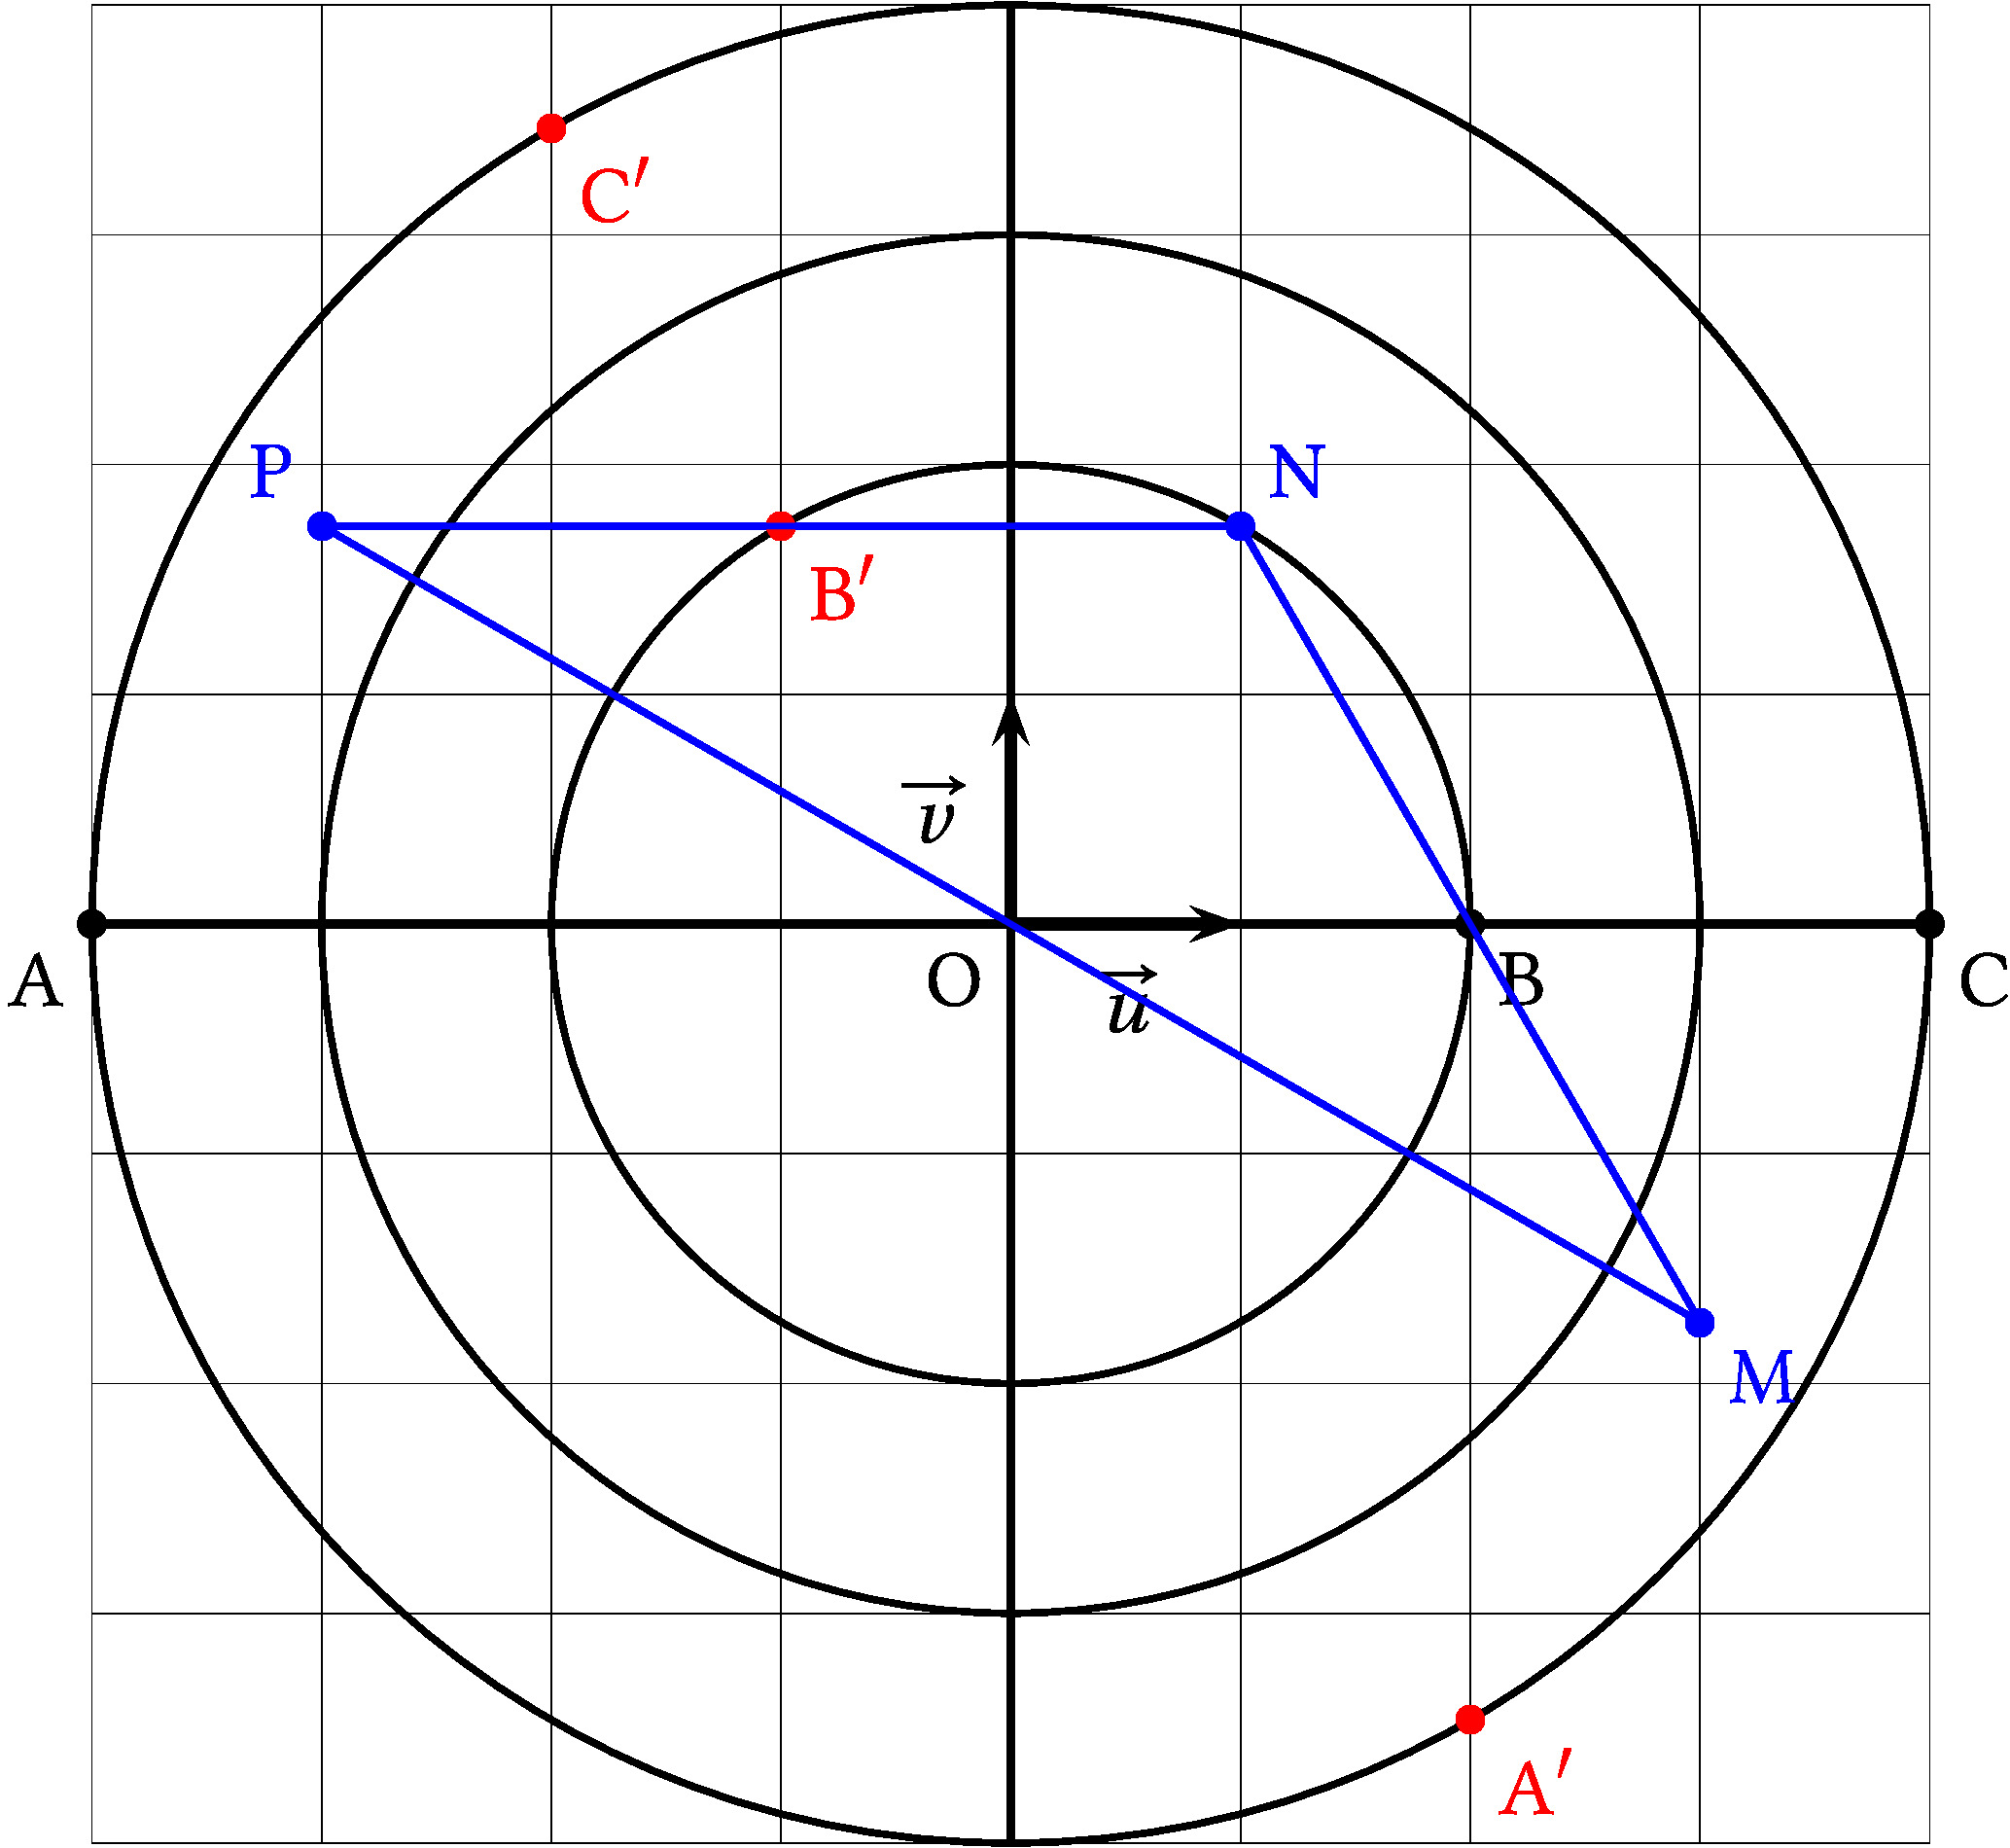
\includegraphics{./TS-Complexes-Loga-0}



$|a'|=4$ donc A$'$ est sur le cercle de centre O et de rayon 4 et on a $Re\left(a' \right) =2$ et $Im\left(a' \right)<0$, on peut donc placer A$'$


$|b'|=2$ donc B$'$ est sur le cercle de centre O et de rayon 2 et on a $Re\left(b' \right) =-1$ et $Im\left(b' \right)>0$, on peut donc placer B$'$


$|c'|=4$ donc C$'$ est sur le cercle de centre O et de rayon 4 et on a $Re\left(c' \right) =-2$ et $Im\left(c' \right)>0$, on peut donc placer C$'$



:::endsolution

\end{enumerate}

\item  Montrer que les points A$'$, B$'$ et C$'$ sont alignés.

\setbar{1}

:::startsolution


$a'=-c'$ donc A$'$ et C$'$ sont symétriques par rapport à O alors O, A$'$ et C$'$ sont alignés

$arg\left( b'\right) =arg\left( c'\right) =\dfrac{2\pi}{3} (2\pi)$

donc $\overrightarrow{\text{OB}'}$ et $\overrightarrow{\text{OC}'}$ sont colinéaires d'où O, B$'$ et C$'$ sont alignés.

Finalement O, A$'$, B$'$ et C$'$ sont alignés.


:::endsolution

\item  On note M le milieu du segment [A$'$C], N le milieu du segment [C$'$C] et P le milieu du
segment [C$'$A].

Démontrer que le triangle MNP est isocèle.

\setbar{1.5}

:::startsolution


$z_{\text{M}}=\dfrac{a'+c}{2}=3-\text{i}\sqrt{3}$

$z_{\text{N}}=\dfrac{c'+c}{2}=1+\text{i}\sqrt{3}$

$z_{\text{P}}=\dfrac{c'+a}{2}=-3+\text{i}\sqrt{3}$

MNP semble isocèle en N d'après le dessin

MN=$\left|z_{\text{N}}-z_{\text{M}} \right| = \left|2-2\text{i}\sqrt{3} \right| =4$

et

PN=$\left|z_{\text{N}}-z_{\text{P}} \right| =\left|4 \right| = 4$

On a MN=NP donc MNP est bien isocèle en N


:::endsolution
\end{enumerate}


\bigskip




\textbf{Graphique à compléter}

\bigskip

\psset{unit=1cm}

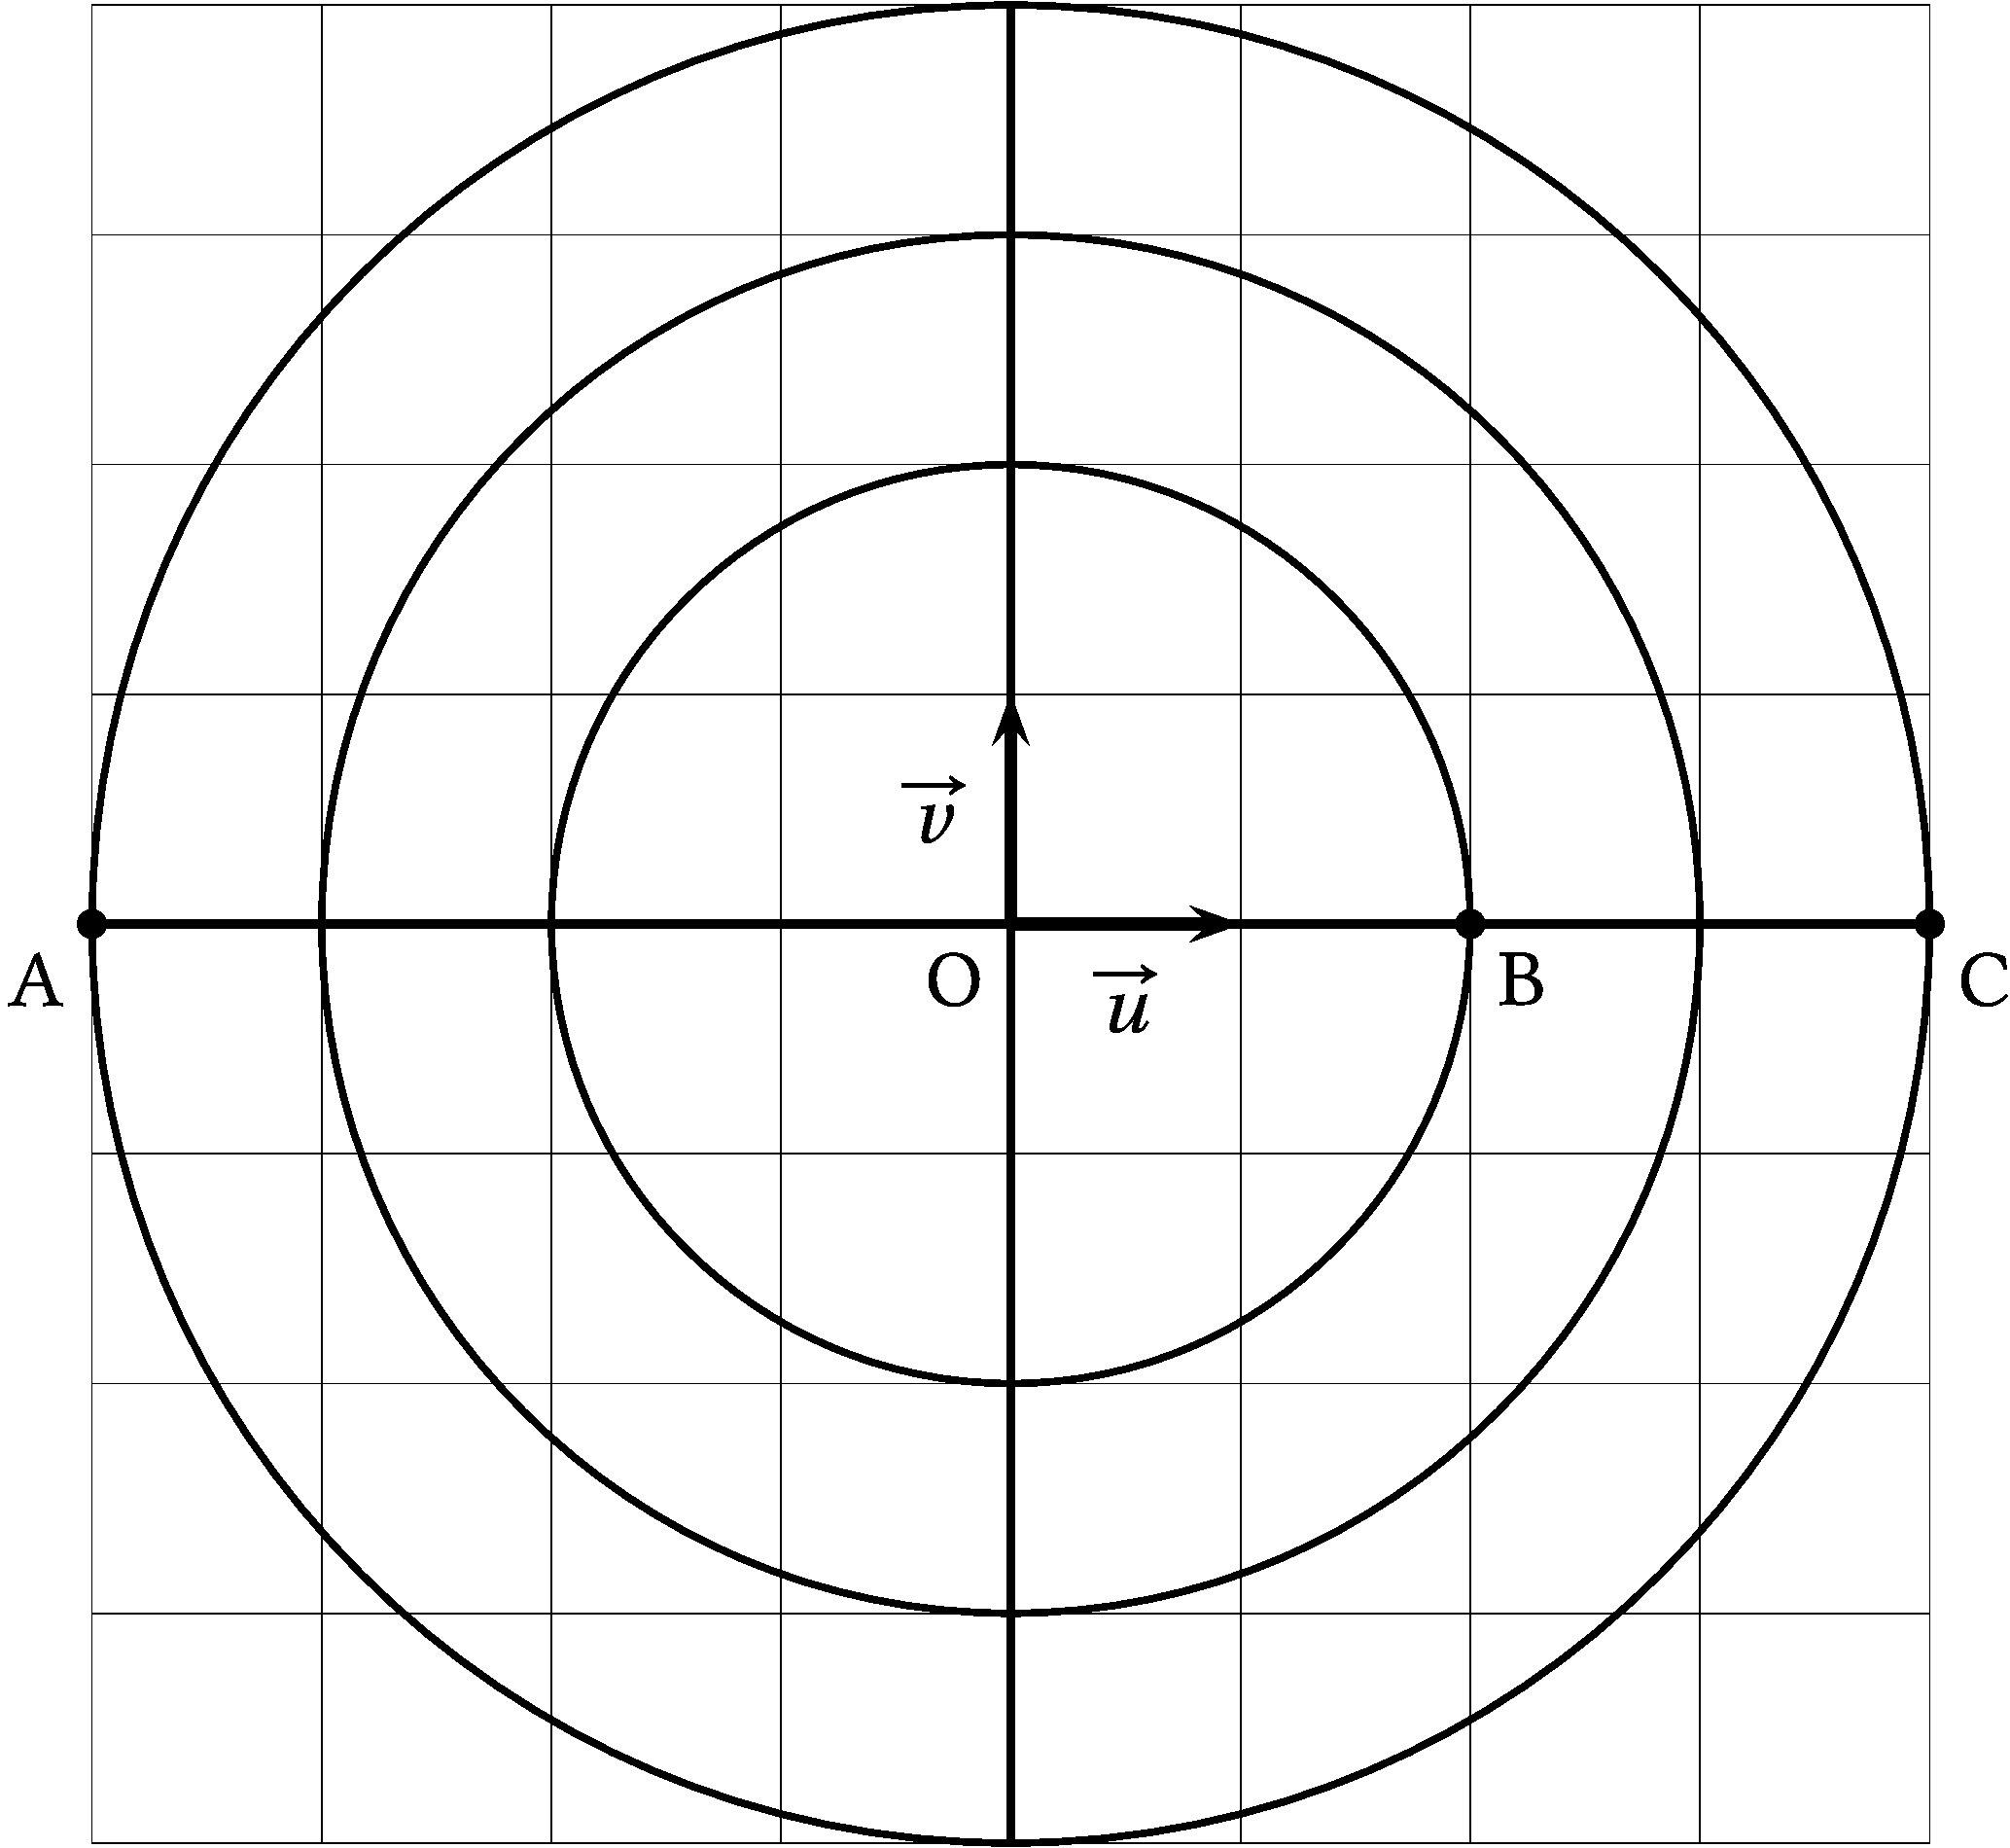
\includegraphics{./TS-Complexes-Loga-1}




:::

\newpage



:::exercice Exercice:

[Un peu de physique, mais pas trop...][10]
Lors d'une expérience en laboratoire, on lance un projectile dans un milieu fluide. L'objectif est de déterminer pour quel angle de tir
$\theta$ par rapport à l'horizontale la hauteur du projectile ne dépasse
pas $1,6$ mètre.

Comme le projectile ne se déplace pas dans l'air mais dans un
fluide, le modèle parabolique usuel n'est pas adopté.

On modélise ici le projectile par un point qui se déplace, dans un
plan vertical, sur la courbe représentative de la fonction $f$ définie
sur l'intervalle [0~;~1[ par:


$$
f(x) = bx + 2\ln (1- x)
$$


où $b$ est un paramètre réel supérieur ou égal à $2$, $x$ est l'abscisse
du projectile, $f(x)$ son ordonnée, toutes les deux exprimées en mètres.



\psset{unit=4cm,comma=true}

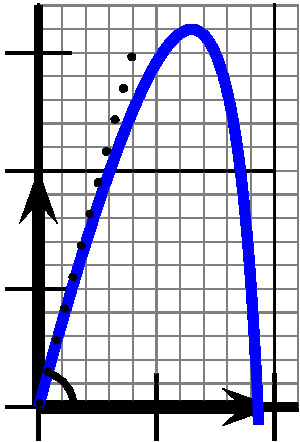
\includegraphics{./TS-Complexes-Loga-2}






\begin{enumerate}
\item La fonction $f$ est dérivable sur l'intervalle [0~;~1[. On note $f'$ sa fonction dérivée.

\begin{enumerate}
\item Démontrer que, pour tout réel
$x$ de l'intervalle [0~;~1[ :


$$
f'(x) = \dfrac{- bx + b - 2}{1 - x}.
$$


\setbar{1}

:::startsolution

On va utiliser: $\left(\ln (u) \right) ' = \frac{u'}{u}$

$f'(x) = b + 2\times \frac{-1}{1-x} = \cdots = \frac{-bx+x-2}{1-x}$


:::endsolution
\item Démontrer que fonction $f$ possède un maximum sur l'intervalle [0~;~1[ et que,

le maximum de la fonction $f$ est égal à $b - 2 + 2\ln \left(\dfrac{2}{b}\right)$.

\setbar{3}

:::startsolution

Puisque la fonction $f$ est dérivable, et que l'on connaît sa fonction dérivée, on va étudier le signe de la fonction dérivée pour connaître les variations de la fonction $f$.

\smallskip

Soit $x$ dans $[0~;~1[$. On a $x < 1$ et donc, $0< 1  -x$.

Le dénominateur de $f'(x)$ étant strictement positif, le signe de $f'(x)$ est le signe du numérateur, qui est une quantité affine, de coefficient directeur $- b$ négatif (puisque $b$ est supérieur à 2) et donc on aura bien une fonction dérivée d'abord positive, pour $x \leqslant \dfrac{b - 2}{b}$, puis négative.

On remarque le nombre $\dfrac{b-2}{b} = 1 - \dfrac{2}{b}$ est un nombre inférieur à 1 et positif, car $b$ est un réel positif, supérieur à 2.

On peut donc affirmer que la fonction $f$ est croissante sur l'intervalle $\left[0~;~\dfrac{b - 2}{b}\right] $ et décroissante sur $\left[\dfrac{b - 2}{b}~;~1\right[$.

Ces variations indiquent que $f$ atteint un maximum pour $x = \dfrac{b - 2}{b} = 1 - \dfrac{2}{b}$.

Ce maximum est donc $f\left(1 - \dfrac{2}{b}\right) = b\times \left(1 - \dfrac{2}{b}\right) + 2\ln\left(1 - \left(1 - \dfrac{2}{b} \right) \right) = b - 2 + 2 \ln\left(\dfrac{2}{b}\right) $.

Le maximum de la fonction $f$ s'établit bien à $b - 2 + 2 \ln\left(\dfrac{2}{b}\right) $.


:::endsolution
\end{enumerate}


\item  On cherche à déterminer pour quelles valeurs du paramètre $b$ la hauteur maximale du projectile ne dépasse
pas $1,6$~mètre.

Si on essaye de résoudre l'inéquation $b - 2 + 2 \ln\left(\dfrac{2}{b}\right) \leqslant 1,6$, on se retrouve devant une équation que l'on ne sait pas résoudre de façon exacte.

Posons $m$ la fonction définie sur $[2~;~+\infty[$ par $m(b) = b - 2 + 2 \ln\left(\dfrac{2}{b}\right) = b - 2 + \ln(4) - 2\ln(b)$.

\begin{enumerate}

\item Etudier les variations de la fonction $m$ pour $b$ supérieur à 2.

\setbar{1.5}

:::startsolution

La fonction $m$ est dérivable sur son ensemble de définition et on a pour tout $b$ supérieur à 2 :

$m'(b) = 1 - \dfrac{2}{b}$.

Comme $b$ est supérieur à 2, on en déduit que $m'(b)$ est positif, et même strictement positif pour $b>2$, et donc que la fonction $m$ est strictement croissante sur $[2~;~+\infty[$.


:::endsolution
\item Déterminer: $\lim_{b \to +\infty} m(b)$

\setbar{1}

:::startsolution

TODO


:::endsolution
\item Dresser le tableau de variation de $m$ sur $[2;+\infty[$

\setbar{0.5}

:::startsolution

TODO


:::endsolution

\item Démontrer que l'équation $m(b)=1,6$ admet une unique solution $b_0$ dans $[2;10]$. En donner un encadrement à $0,01$ près.

\setbar{1.5}

:::startsolution

La fonction $m$ étant continue (car dérivable) et strictement croissante sur l'intervalle $[2~;~10]$ et 1,6 étant une valeur intermédiaire entre $m(0) = 0$ et $m(10) \approx 4,8$, le corollaire au théorème des valeurs intermédiaires permet d'affirmer qu'il existe un unique nombre $b_0$ antécédent de 1,6 par $m$ sur $[2~;~10]$. Comme $m$ est strictement croissante sur $[2~;~+\infty[$, il n'y aura pas d'autre antécédent que celui là.

Un balayage à la calculatrice donne $5,69 < b_0 < 5,70$.


:::endsolution
\item Conclure.

\setbar{0.5}

:::startsolution


Les valeurs du paramètre $b$ garantissant une hauteur maximale $m(b)$ ne dépassant pas 1,6 mètre sont donc les réels de l'intervalle $[2~;~b_0]$, soit, en donnant une valeur approchée (nécessairement par défaut, vu que $m$ est croissante) de l'intervalle $[2~;~5,69]$.


:::endsolution
\end{enumerate}



\setcounter{enumii}{0}
\item  Dans cette question, on choisit $b = 5,69$.

L'angle de tir $\theta$ correspond à l'angle entre l'axe des abscisses et la tangente à la courbe de la
fonction $f$ au point d'abscisse $0$ comme indiqué sur le schéma donné ci-dessus.

Déterminer une valeur approchée au dixième de degré près de l'angle $\theta$.

\setbar{1}

:::startsolution

Si on choisit $b = 5,69$, alors, cela signifie que la tangente tracée en pointillés est la droite d'équation :

$$
y = f'(0) \times (x - 0) + f(0) = \dfrac{b - 2}{1 - 0} \times x + 0 = (5,69 - 2)x = 3,69x
$$

Cela signifie que l'origine du repère, le point de coordonnée $(1~;~0)$ et le point de coordonnées $(1~;~3,69)$ forment un triangle rectangle, dans lequel le côté opposé à l'angle $\theta$ mesure 3,69 et le côté adjacent mesure $1$, donc la tangente de l'angle est donnée par $\tan \theta = \dfrac{3,69}{1} = 3,69$.

À la calculatrice (réglée en mode degrés), on obtient $\theta = \arctan(3,69) \approx 74,8$ degrés


:::endsolution
\end{enumerate}

:::



:::exercice Exercice:

[VRAI-FAUX][4]
Pour chacune des  affirmations suivantes,
indiquer si elle est vraie ou fausse,
en justifiant la réponse.
Il est attribué deux points par réponse exacte correctement justifiée.



\begin{enumerate}

\item  On considère dans $\R$ l'équation :


$$
\ln (6 x - 2) + \ln (2x - 1) = \ln (x).
$$




\textbf{Affirmation} l'équation admet deux solutions dans l'intervalle $\left]\dfrac{1}{2}~;~+ \infty\right[$.

\setbar{2}

:::startsolution


\begin{list}{\textbullet}{}
\item Soit $I=\left]\frac{1}{2}~;~+ \infty\right[$.

\begin{list}{$\circ$}{}
\item $\ln\left (6x-2\right )$ n'existe que si $6x-2>0$, c'est-à-dire $x>\dfrac{1}{3}$; donc $\ln\left (6x-2\right )$ existe si $x\in I$.
\item $\ln\left (2x-1\right )$ n'existe que si $2x-1>0$, c'est-à-dire $x>\dfrac{1}{2}$; donc $\ln\left (2x-1\right )$ existe si $x\in I$.
\item $\ln\left (x\right )$ n'existe que si $x>0$; donc $\ln\left (x\right )$ existe si $x\in I$.
\end{list}

\item Sur l'intervalle $I$:

$\ln (6 x - 2) + \ln (2x - 1) = \ln (x)
\iff \ln \left ((6 x - 2)(2x - 1)\strut\right ) = \ln (x)
\iff  (6 x - 2)(2x - 1) = x \newline
\iff 12x^2 - 4x - 6x + 2 = x
\iff 12x^2 -11x +2=0$
\item On résout dans $I$ l'équation $12x^2 -11x +2=0$.

$\Delta = 11^2 - 4\times 12\times 2 = 25 = 5^2$;
$x'=\dfrac{11+5}{2\times 12} = \dfrac{16}{24}=\dfrac{2}{3}$ et
$x''=\dfrac{11-5}{24}=\dfrac{6}{24}= \dfrac{1}{4}$

$x'\in I$ et $x'' \not\in I$ donc l'équation du départ n'admet qu'une solution dans l'intervalle $I$.
\end{list}

\textbf{L'affirmation est fausse.}


:::endsolution
\item  On considère dans \mathcal{C} l'équation :


$$
\left(4z^2 - 20z + 37\right)(2z -7 + 2\text{i}) = 0.
$$




\textbf{Affirmation} les solutions de l'équation sont les affixes de points appartenant à un même
cercle de centre le point P d'affixe $2$.

\setbar{2}

:::startsolution


\begin{list}{\textbullet}{}
\item Les solutions de l'équation $\left(4z^2 - 20z + 37\right)(2z -7 + 2i) = 0$ sont les solutions des deux équations $4z^2 - 20z + 37 = 0$ et $2z -7 + 2i = 0$.
\item On résout dans \mathcal{C} l'équation $4z^2 - 20z + 37 = 0$.

$\Delta=20^2 - 4\times 4\times 37 = -192<0$; l'équation admet donc deux solutions complexes conjuguées:
$z_1 = \dfrac{20 + i \sqrt{192}}{2\times 4} = \dfrac{20 + 8i \sqrt{3}}{8} = \dfrac{5}{2}+i\sqrt{3}$ et $z_2 = \dfrac{5}{2} - i\sqrt{3}$

\item On résout dans \mathcal{C} l'équation $2z-7+2i=0$:
$2z-7+2i=0 \iff 2z=7-2i \iff z = \dfrac{7}{2} - i$

Cette équation a pour solution le nombre complexe $z_3=\dfrac{7}{2}- i$.

\item On appelle  A, B et C les points d'affixes respectives $z_1$, $z_2$ et $z_3$.


\begin{list}{$\circ$}{}
\item $\mathrm{PA} = \left |  z_1 - z_{\mathrm{P}} \right | = \left | \dfrac{5}{2} + i\sqrt{3} -2 \right | = \left |  \dfrac{1}{2} +i\sqrt{3} \right | = \ds\sqrt{\dfrac{1}{4} + 3} = \sqrt{\dfrac{13}{4}}$
\item $\mathrm{PB} = \left |z_2 - z_{\mathrm{P}} \right | = \left |\dfrac{5}{2} - i\sqrt{3}-2 \right | = \left |  \dfrac{1}{2} - i\sqrt{3} \right | = \sqrt{\dfrac{1}{4} + 3} = \sqrt{\dfrac{13}{4}}$
\item $\mathrm{PC} = \left | z_3 - z_{\mathrm{P}} \right | = \left |\dfrac{7}{2} - i -2 \right | = \left | \dfrac{3}{2} - i \right | = \sqrt{\dfrac{9}{4} + 1} = \sqrt{\dfrac{13}{4}}$
\end{list}


\item $\mathrm{PA} = \mathrm{PB} = \mathrm{PC}$ donc les solutions de l'équation sont les affixes de trois points situés sur le cercle de centre P d'affixe 2 et de rayon $\dfrac{13}{4}$.

\end{list}

\textbf{L'affirmation est vraie.}


:::endsolution
\end{enumerate}

:::



:::exercice Exercice:

[Complexes: suites...][10.5]
Le plan complexe est muni d'un repère orthonormé direct $\left(\text{O};~\overrightarrow{u},~\overrightarrow{v}\right)$.

On pose $z_0 = 8$ et, pour tout entier naturel $n$ :


$$
z_{n+1} = \dfrac{3 - \text{i}\sqrt{3}}{4}z_n.
$$


On note $A_n$ le point du plan d'affixe $z_n$.

\medskip


\begin{enumerate}
\item

\begin{enumerate}
\item Vérifier que :


$$
\dfrac{3 - \text{i}\sqrt{3}}{4} = \dfrac{\sqrt{3}}{2}\text{e}^{- \text{i}\frac{\pi}{6}}.
$$


\setbar{0.5}

:::startsolution

$\dfrac{\sqrt{3}}{2} \text{e}^{-\text{i} \frac{\pi}{6}} = \dfrac{\sqrt{3}}{2} \left( \cos\left(-\dfrac{\pi}{6}\right) + \text{i}\sin\left(-\dfrac{\pi}{6}\right) \right) = \dfrac{\sqrt{3}}{2} \left( \dfrac{\sqrt{3}}{2} - \text{i}\dfrac{1}{2} \right) = \dfrac{3}{4} - \text{i} \dfrac{\sqrt{3}}{4} = \dfrac{3-\text{i}\sqrt{3}}{4}$


:::endsolution
\item En déduire l'écriture de chacun des nombres complexes $z_1$,  $z_2$ et $z_3$ sous forme exponentielle et vérifier que $z_3$ est un imaginaire pur dont on précisera la partie imaginaire.

\setbar{2}

:::startsolution

$z_1=\dfrac{\sqrt{3}}{2} \text{e}^{-\text{i} \frac{\pi}{6}}z_0=\dfrac{\sqrt{3}}{2} \text{e}^{-\text{i} \frac{\pi}{6}} \times 8$ donc $\boxed{ z_1=4\sqrt{3} \text{e}^{-\text{i} \frac{\pi}{6}} }$\smallskip

$z_2=\dfrac{\sqrt{3}}{2} \text{e}^{-\text{i} \frac{\pi}{6}}z_1 = \dfrac{\sqrt{3}}{2} \text{e}^{-\text{i} \frac{\pi}{6}} \times 4\sqrt{3} \text{e}^{-\text{i} \frac{\pi}{6}} = 6 \text{e}^{-\text{i} \frac{2\pi}{6}}$ donc $\boxed{ z_2=6 \text{e}^{-\text{i} \frac{\pi}{3}} }$\smallskip

$z_3=\dfrac{\sqrt{3}}{2} \text{e}^{-\text{i} \frac{\pi}{6}}z_2 = \dfrac{\sqrt{3}}{2} \text{e}^{-\text{i} \frac{\pi}{6}} \times 6 \text{e}^{-\text{i} \frac{\pi}{3}} = 3\sqrt{3} \text{e}^{-\text{i} \frac{3\pi}{6}}$ donc $\boxed{ z_3=3\sqrt{3} \text{e}^{-\text{i} \frac{\pi}{2}} }$\medskip

$\arg(z_3) = \dfrac{-\pi}{2}$ donc $z_3$ est un imaginaire pur dont la partie imaginaire est négative et

$\boxed{ \text{Im}\left(z_3\right) = - 3\sqrt{3} }$


:::endsolution
\item Représenter graphiquement les points $A_0$ , $A_1$ , $A_2$ et $A_3$ ; on prendra pour unité le centimètre.

\setbar{2}

:::startsolution

\textsc{Figure représentation des points $A_0$, \:$A_1$, \:$A_2$, \:$A_3$}

La relation $z_{n+1} = \dfrac{\sqrt{3}}{2}\text{e}^{- \text{i}\frac{\pi}{6}}z_n$ montre en prenant les arguments que

arg$\left(z_{n+1} \right) = \text{arg}\left(\dfrac{\sqrt{3}}{2}\text{e}^{- \text{i}\frac{\pi}{6}}\right) + \text{arg}\left(z_n\right)$.
Or $\text{arg}\left(\dfrac{\sqrt{3}}{2}\text{e}^{- \text{i}\frac{\pi}{6}} \right) = - \dfrac{\pi}{6}$.

On a donc pour tout $n \in \N$, $\left(\overrightarrow{\text{O}A_n},~\overrightarrow{\text{O}A_{n+1}} \right) = - \dfrac{\pi}{6}$.

On a donc $\left(\overrightarrow{\text{O}A_0},~\overrightarrow{\text{O}A_{1}} \right) = - \dfrac{\pi}{6}$, puis
$\left(\overrightarrow{\text{O}A_0},~\overrightarrow{\text{O}A_{2}} \right) = - \dfrac{\pi}{3}$ et $\left(\overrightarrow{\text{O}A_0},~\overrightarrow{\text{O}A_{3}} \right) = - \dfrac{\pi}{2}$.

\smallskip

$\bullet~~$$A_0$ a pour affixe 8 ;

$\bullet~~$ On sait que $\sin - \frac{\pi}{6} = - \frac{1}{2}$. On trace donc l'horizontale partant du point de coordonnées $(0~;~- 4)$ qui coupe le cercle de centre O de rayon 8 en un point B d'abscisse positive. La droite verticale d'équation $x = 6$ coupe OB en $A_1$.

$\bullet~~$ On sait que $\cos - \frac{\pi}{3} =  \frac{1}{2}$. On trace donc la verticale ale partant du point de coordonnées $(4~;~0)$ qui coupe le cercle de centre O de rayon 8 en un point C d'ordonnée négative. La droite verticale  d'équation $x = 3$ coupe OC en $A_2$.

$\bullet~~$ Enfin $A_3$ est le projeté orthogonal de $A_2$ sur l'axe des ordonnées puisque $\text{O}A_3 = \dfrac{\sqrt{3}}{2}\text{O}A_2$ ou encore $\text{O}A_3 = \cos \frac{\pi}{6}\text{O}A_2$.


\psset{unit=1cm}

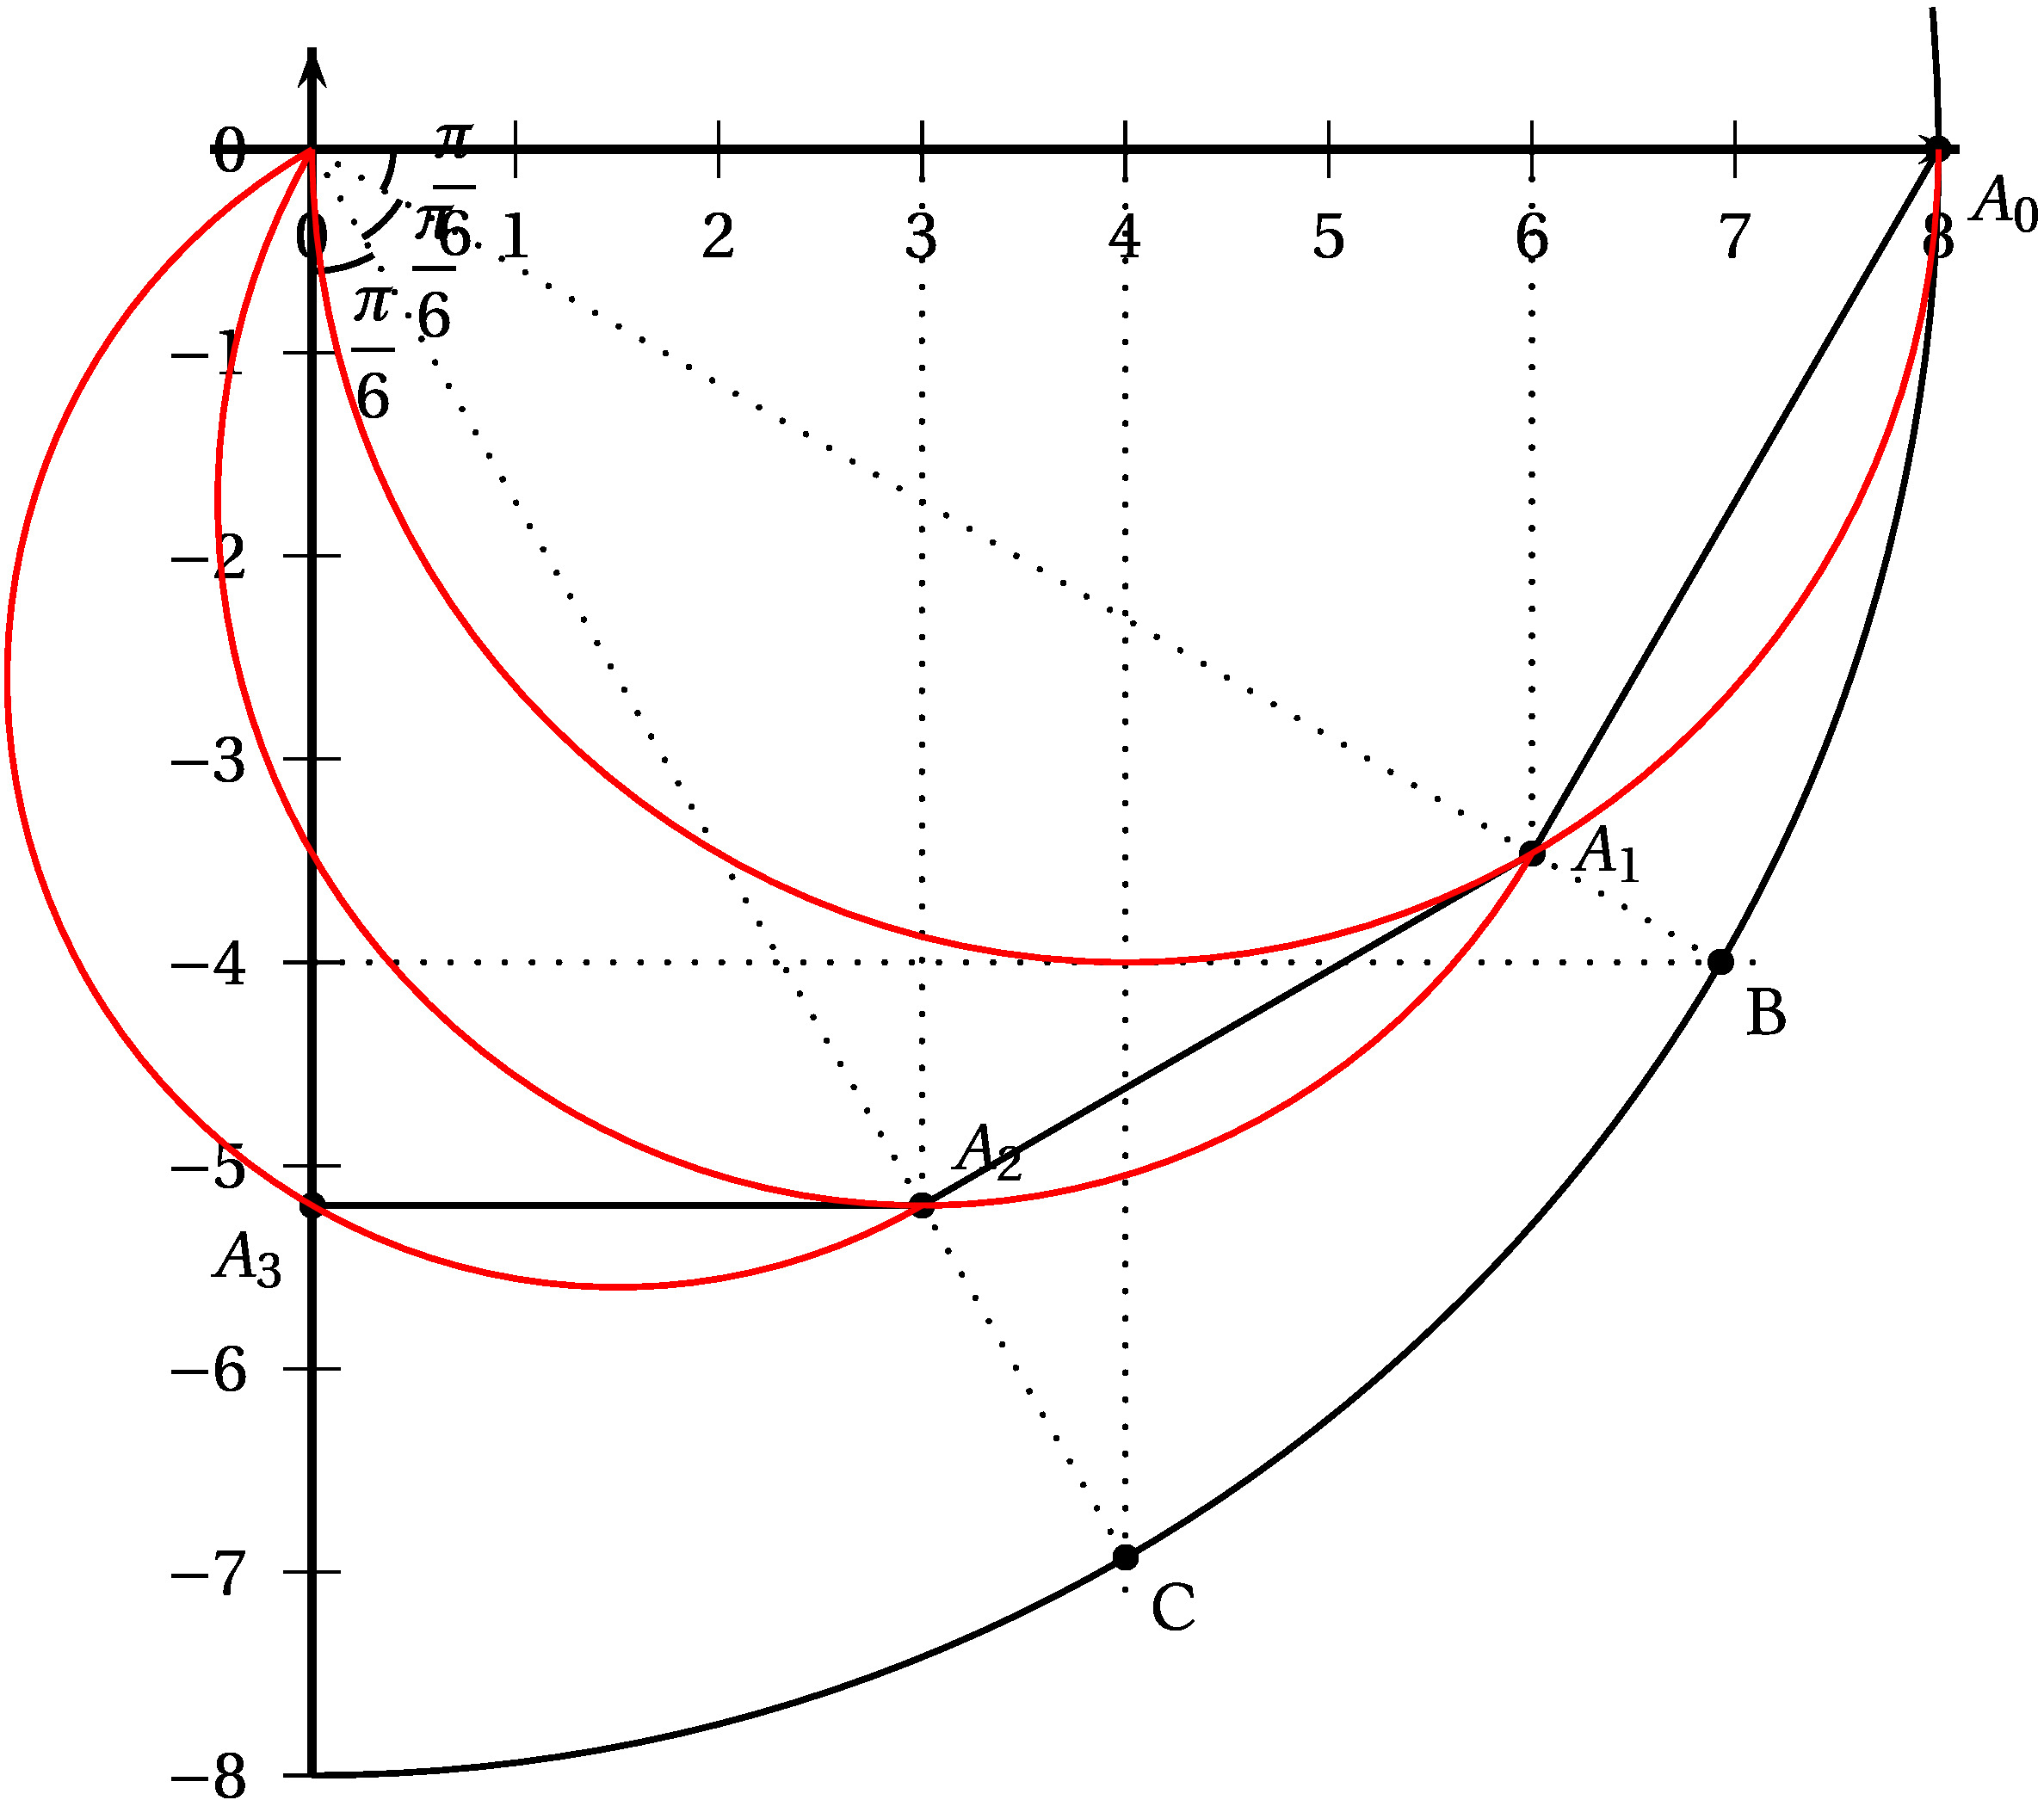
\includegraphics{./TS-Complexes-Loga-3}




\smallskip

\emph{Remarque} :

Puisque que pour tout naturel $n$, \: O$A_{n+1} = \cos \frac{\pi}{6} \text{O}A_n$, le point $A_{n+}$ est la projeté orthogonal de $A_n$ sur la droite O$A_{n+1}$.

$A_1$ est donc le point d'intersection de la droite (OB) avec le demi-cercle de diamètre $\left[\text{O}A_0\right]$ contenant les points d'ordonnée négative.

$A_2$ est le point d'intersection de la droite (OC) avec le demi-cercle de diamètre $\left[\text{O}A_1\right]$. (voir les demi-cercles tracés en rouge)

$A_3$ est le point d'intersection de l'axe des ordonnées  avec le demi-cercle de diamètre $\left[\text{O}A_2\right]$.


:::endsolution
\end{enumerate}

\item

\begin{enumerate}
\item Démontrer par récurrence que, pour tout entier naturel $n$,


$$
z_n = 8 \times \left(\dfrac{\sqrt{3}}{2}\right)^n \text{e}^{- \text{i}\frac{n\pi}{6}}.
$$


\setbar{1.5}

:::startsolution

\emph{Initialisation} $z_0 = 8 \times 1 \times 1 = 8$ donc la propriété est vraie pour $n=0$.\smallskip

\emph{Hérédité} : On suppose que pour $n \geqslant 0$,  $z_n=8 \times \left( \dfrac{\sqrt{3}}{2} \right)^n \text{e}^{-\text{i} \frac{n\pi}{6}}$ et on va montrer que

$z_{n+1} = 8 \times \left( \dfrac{\sqrt{3}}{2} \right)^{n+1} \text{e}^{-\text{i} \frac{(n+1)\pi}{6}}$\medskip

On a $z_{n+1}= \dfrac{\sqrt{3}}{2} z_n= \dfrac{\sqrt{3}}{2}\text{e}^{-\text{i} \frac{\pi}{6}} \times 8\times \left( \dfrac{\sqrt{3}}{2} \right)^n \text{e}^{-\text{i} \frac{n\pi}{6}}$ \textit{(par hypothèse de récurrence)}.\smallskip

Donc $z_{n+1}=8 \times \left( \dfrac{\sqrt{3}}{2} \right)^{n+1} \text{e}^{-\text{i} \frac{(n+1)\pi}{6}}$ \textit{ (en utilisant la propriété $a^n \times a = a^{n+1}$ pour tout nombre réel $a$) }.\smallskip

Donc la propriété est héréditaire.\smallskip

La propriété est vraie au rang $0$, et si elle est vraie au rang $n \geqslant 0$, elle l'est aussi au rang $n + 1$

Conclusion : d'après le principe de récurrence la propriété est vraie pour tout entier naturel $n$.


:::endsolution
\item Pour tout entier naturel $n$, on pose $u_n = \left|z_n\right|$.

Déterminer la nature et la limite de la suite $\left(u_n\right)$.

\setbar{1.5}

:::startsolution

On a donc $u_n=\left|z_n\right| =8 \times \left( \dfrac{\sqrt{3}}{2} \right)^n$\smallskip

Il s'agit d'une suite géométrique de premier terme $u_0=8$ et de raison $\dfrac{\sqrt{3}}{2}$. \medskip

$0 < \dfrac{\sqrt{3}}{2} < 1$ donc $\displaystyle\lim_{n \to + \infty} \left( \dfrac{\sqrt{3}}{2} \right)^n = 0$ puis $\boxed{ \displaystyle\lim_{n \to + \infty} u_n = 8 \times 0 = 0 }$


:::endsolution
\end{enumerate}

\item

\begin{enumerate}
\item Démontrer que, pour tout entier naturel $k$,


$$
\dfrac{z_{k+1} - z_{k}}{z_{k+1}} = - \dfrac{1}{\sqrt{3}}\text{i}.
$$


En déduire que, pour tout entier naturel $k$, on a l'égalité : $A_kA_{k+1} = \dfrac{1}{\sqrt{3}} \text{O}A_{k+1}$.

\setbar{1.5}

:::startsolution

$\dfrac{z_{k+1} - z_k}{z_{k+1} } = \dfrac{ \dfrac{3-\text{i}\sqrt{3}}{4}z_k - z_k}{ \dfrac{3-\text{i}\sqrt{3}}{4}z_k } = \dfrac{ \cancel{z_k} \left( \dfrac{3-\text{i}\sqrt{3}}{4} - 1 \right)}{ \dfrac{3-\text{i}\sqrt{3}}{4}\cancel{z_k} }
=\dfrac{ \dfrac{3-\text{i}\sqrt{3}}{4} - 1 }{\dfrac{3-\text{i}\sqrt{3}}{4}}
= \dfrac{ -1-\text{i}\sqrt{3} }{4} \times \dfrac{4}{3-\text{i}\sqrt{3}}
= \dfrac{ -1-\text{i}\sqrt{3} }{3-\text{i}\sqrt{3}}$\medskip

On multiplie par le conjugué du dénominateur :\smallskip

$\dfrac{z_{k+1} - z_k}{z_{k+1}}
=\dfrac{ (-1-\text{i}\sqrt{3})(3+\text{i}\sqrt{3}) }{ (3-\text{i}\sqrt{3})(3+\text{i}\sqrt{3})}
= \dfrac{-3-\text{i}\sqrt{3}-3\text{i}\sqrt{3}+3 }{9+3} = \dfrac{-4\text{i}\sqrt{3}\times \sqrt{3} }{12 \times \sqrt{3} } = \dfrac{-12\text{i}}{12\sqrt{3}} = - \dfrac{1}{\sqrt{3}} \text{i}$\medskip

On a donc $\left|\dfrac{z_{k+1} - z_k}{z_{k+1} }\right| = \left|- \dfrac{1}{\sqrt{3}} \text{i}\right|
\iff \dfrac{\left|z_{k+1} - z_k \right|}{\left|z_{k+1} \right|} = \dfrac{1}{\sqrt{3}}
\iff \dfrac{A_kA_{k+1}}{OA_{k+1}} = \dfrac{1}{\sqrt{3}}
\iff $

$A_kA_{k+1} = \dfrac{1}{\sqrt{3}} OA_{k+1}$.


:::endsolution
\item Pour tout entier naturel $n$, on appelle $\ell_n$ la longueur de la ligne brisée reliant dans cet ordre les points $A_0$,\: $A_1$,\: $A_2$, \ldots , $A_n$.

On a ainsi : $\ell_n = A_0A_1 + A_1A_2 + \ldots + A_{n-1}A_n$.

Démontrer que la suite $\left(\ell_n\right)$ est convergente et calculer sa limite.

\setbar{1.5}

:::startsolution

D'après la question précédente, pour tout entier naturel $k$,\smallskip

$A_kA_{k+1} = \dfrac{1}{\sqrt{3}} OA_{k+1} = \dfrac{1}{\sqrt{3}} \left|z_{k+1} \right| = \dfrac{1}{\sqrt{3}} \times 8 \times \left( \dfrac{\sqrt{3}}{2} \right)^{k+1} = \dfrac{8}{\sqrt{3}} \left( \dfrac{\sqrt{3}}{2} \right)^{k+1}$ \medskip

Donc $\ell_n=\dfrac{8}{\sqrt{3}} \left( \dfrac{\sqrt{3}}{2} \right)^1 + \dfrac{8}{\sqrt{3}} \left( \dfrac{\sqrt{3}}{2} \right)^2 + \cdots + \dfrac{8}{\sqrt{3}} \left( \dfrac{\sqrt{3}}{2} \right)^n
= \dfrac{8}{\sqrt{3}} \times \dfrac{\sqrt{3}}{2} \left( 1 +  \left( \dfrac{\sqrt{3}}{2} \right)^1 + \cdots + \left( \dfrac{\sqrt{3}}{2} \right)^{n-1} \right)$\medskip

Puis $\ell_n=4 \times \dfrac{1 - \left( \dfrac{\sqrt{3}}{2} \right)^{n} }{1-\left( \dfrac{\sqrt{3}}{2} \right)}
=4 \times \dfrac{1 - \left( \dfrac{\sqrt{3}}{2} \right)^{n} }{\dfrac{2-\sqrt{3}}{2}}
=\dfrac{8}{2-\sqrt{3}} \times \left( 1 - \left( \dfrac{\sqrt{3}}{2} \right)^{n} \right)$\medskip

Pour finir, $\displaystyle\lim_{n \to + \infty} \ell_n=\dfrac{8}{2-\sqrt{3}}(1-0) =\dfrac{8}{2-\sqrt{3}} \approx 29,86$


:::endsolution
\end{enumerate}

\end{enumerate}

:::





\end{document}